\documentclass[a4paper]{article}
\usepackage{amsmath, amsfonts, amssymb, amsthm}
\usepackage{booktabs}
\usepackage{color}
\usepackage{comment}
\usepackage{enumitem}
\usepackage[top=2cm,bottom=2cm,left=3cm,right=3cm]{geometry}
\usepackage{graphicx}
\usepackage{hyperref}
\usepackage{listings}
\usepackage{tikz}
\usepackage{url}
\usepackage{lineno}
\usepackage{xspace}
\usepackage{biblatex} % Added for citations
\addbibresource{citations.bib} % Path to your citations.bib file

%%% TIKZ
\usetikzlibrary{calc}
\usetikzlibrary{decorations}
\usetikzlibrary{positioning}
\usetikzlibrary{shapes}

%%% STYLE
\renewcommand{\familydefault}{\sfdefault}
\setlength\parindent{0pt}

%%% ENVIRONMENTS

% Question environment
\newtheoremstyle{que}% name
  {}% Space above, empty = `usual value'
  {}% Space below
  {}% Body font
  {}% Indent amount (empty = no indent, \parindent = para indent)
  {\bfseries}% Thm head font
  {}% Punctuation after thm head
  {\newline}% Space after thm head: \newline = linebreak
  {\thmname{#1}\thmnumber{ #2}:\thmnote{ #3}\vspace{\medskipamount}}% Thm head spec
\theoremstyle{que}
\newtheorem{question}{Question}

%%% MACROS

% Use to fix offset if an environment starts with an enumerate
\newcommand{\fixoffset}{\mbox{}\vspace*{-\bigskipamount}\vspace*{-\medskipamount}}
\newcommand{\eg}{{\em e.g.}\xspace}
\newcommand{\ie}{{\em i.e.}\xspace}
\mathchardef\mhyphen="2D
\newcommand\points[1]{%
\ifnum1<0#1\relax%
    {\bf \small [#1~marks]}%
  \else%
    {\bf \small [#1~mark]}%
  \fi%
}%

\newcommand{\module}{COMP0143: Cryptocurrencies}
\newcommand{\university}{University College London}
\newcommand{\assessment}{Coursework}
\newcommand{\releaseDate}{November 8, 2024}
\newcommand{\dueDate}{December 11, 2024 at 16:00 UK time}
\newcommand{\feedbackDate}{TBD}
\newcommand{\weight}{40\%}
\newcommand{\pointsTotal}{100 marks}

\begin{document}

\title{\module\\[0.25cm]\assessment}
\author{\university}
\date{Released: \releaseDate\\[0.25cm]Due: \dueDate}
\maketitle

\newpage

%%%%%%%%%%%%%%%%%%%%%%%%%%%%%%%%%%%%%%%%%%%%%%%%%

\begin{question}[\points{25}]
  \fixoffset
  \begin{enumerate}[label=(\alph*)]
    \item 
    \item[(i)] To compute \( C \), we first hash our leaves, the elements of \( S \), to get \( H_1, \ldots, H_9 \). We can then compute the internal nodes \( H_{10}, H_{11}, H_{12} \) as follows:
\[
H_{10} = \text{H}(H_1 || H_2 || H_3)
\]
\[
H_{11} = \text{H}(H_4 || H_5 || H_6)
\]
\[
H_{12} = \text{H}(H_7 || H_8 || H_9)
\]
Finally, \( C \) can be calculated as:
\[
C = H_{13} = \text{H}(H_{10} || H_{11} || H_{12})
\]
A figure \ref{fig:merkle_tree} shows the full Merkle Tree.
\begin{figure}[h!]
    \centering
    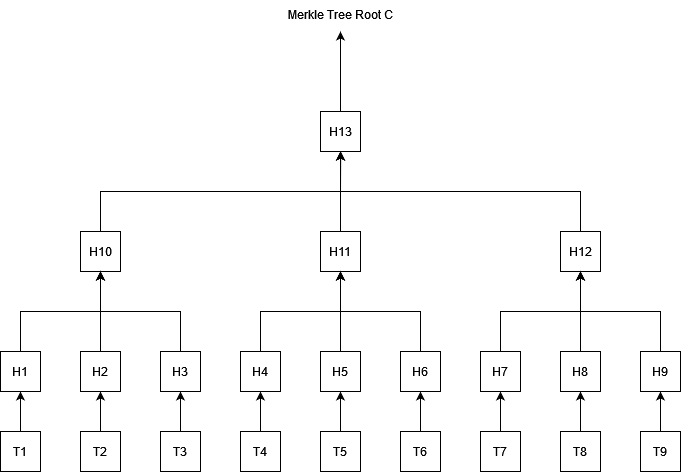
\includegraphics[width=0.5\textwidth]{Merkle Tree example.drawio.png} % Adjust the width as needed
    \caption{Merkle Tree Structure}
    \label{fig:merkle_tree}
To prove \( t_4 \) is in \( S \) we can compute the Merkle Proof as follows:
\[
C = \text{H}(H_{10}||\text{H}(\text{H}(t_4)||H_5||H_6)||H_{12})
\]

\end{figure}
    \item[(ii)] Calculating the Merkle Proof Length \(l\) to show \(t_i\) is in \(S\) is the same as finding the height of the tree. From Merkle root to the hashed leaves the number of nodes increases by a multiple of \(m\) so we can calculate the length as \[m^{l-1} = n \rightarrow \log_m n = l - 1\] As \(n\) may not be a multiple of \(m\) we need to take the ceiling of this value and account for the extra hash on input set here shown using \(l-1\). \[ l = \left\lceil \log_m n \right\rceil + 1\]
    
    \item[(iii)] To minimize the length of the Merkle Proof for a Binary and Ternary Tree we can model the lengths respectively as \[ l = \left\lceil \log_2 n \right\rceil + 1\] and \[ l = \left\lceil \log_3 n \right\rceil + 1\]
    Taking values of n we can compare to see how the functions act for large values. Shown in table \ref{table:two_column_blank} we can see that Ternary Merkle Trees produce smaller Merkle Proofs.
    \begin{table}[h!]
    \centering
    \begin{tabular}{|c|c|c|}
    \hline
    \textbf{N} & \textbf{Binary Merkle Proof Length} & \textbf{Tenary Merkle Proof Length} \\ 
    \hline
             1000 &  11 &   8   \\ 
    \hline
                  10,000  &  15 &    10            \\ 
    \hline
                100,000     & 18  &      12          \\ 
    \hline
               1,000,000      &  21  &       14        \\ 
    \hline
    \end{tabular}
    \caption{Comparison of length of Merkle Proof for Binary and Tenary trees}
    \label{table:two_column_blank}
    \end{table}
    
    \item Merkle Root hashes are included within the blocks within bitcoin as it provides a logarithmic method to check if a transaction is included in a block this was shown in previous question. This is more efficient than the linear method of checking each transaction in the full list individually. The impact of not including this would be a decrease in the efficiency of the network as more computations would need to take place to verify inclusion of transactions and each node would need to download the full list of transactions increasing storage. 

    \item 
    
    \item[(i)] The privacy coin chosen for this question is Secret Coin \cite{secret_network_graypaper} this was chosen as it uses a unique concept of secret contracts as smart contracts which allows programmable privacy. The aim of the coin is to keep the functionality of the contracts secret while allowing transaction outcome and validity through public ledgers. This is achieved through the use of Trusted Execution Environment(TEE) which ensures that the data is kept , processed and protected in a trusted environment. Encryption functions such as HKDF-SHA256 and HMAC-SHA256 are used to secure contract states by use of unforgable contract keys derived from the signer's ID and functions can be used to alter the state of the contract. Zero knowledge proofs are used to validate contract execution which protects sensitive data. SCRT tokens are used as the currency and help provide governance through proof of stake. \cite{secret_foundation_docs}
    
    \item[(ii)] In theory, mechanisms such as TEE within secret coin ensure privacy by protecting sensitive data within secret contracts. The network also uses encryption methods to maintain integrity. Proof of stake and public ledger helps ensure validity within the system. However in practice some of the mechanisms are vulnerable. The greypaper \cite{secret_network_graypaper} states some methods of attack including methods to deanonymise users and circumvent validity, showing these are known to the developers. Research on other coins using TEE has found that it is susceptible to side channel attacks and loss of data through TEE crashes \cite{lind2017teechain}. A strength of the TEE is encrypted staking transactions which allows proof of stake without potential to link user identity. The use of encryption methods further helps achieve privacy goals by adding an extra layer of protection to transactions. This is effective for current cryptographic standards but through expansion of network infrastructure or future developments in cryptography , such as quantum cryptography \cite{pirandola2020advances} , could weaken the effectiveness of the privacy.
    
    \item[(iii)]
    An engineering design choice that could help achieve this goal is alternative consensus mechanism. A paper from 2019 highlights some alternative consensus methods for privacy such as Hyperledger \cite{pahlajani2019survey}. As a method to achieve purely privacy this could be effective but could come at a trade off for reduced scalability. One major restriction of secret coin is the use of Intel-SGX for TEE. Alternative hardware implementations could improve privacy by providing a more distributed attack surface, preventing attackers from targeting specific hardware. A non-engineering design choice that could be added is penalties for privacy breaches. Methods such as penalizing validators who do not protect anonymity of transactions could have stashed tokens removed.
    These are a few design choices that could improve the privacy and anonymity of the secret coin network.
  \end{enumerate}
\end{question}

\newpage

%%%%%%%%%%%%%%%%%%%%%%%%%%%%%%%%%%%%%%%%%%%%%%%%%

\begin{question}[\points{25}]
  \fixoffset
  \begin{enumerate}[label=(\alph*)]
    \item When two miners discover the same block simultaneously, both will broadcast their blocks along the network. Other miners will start mining a new block on the chain of the one received first. After some time has passed one of these chains will grow longer than the other, allowing the network to reach consensus on which block is valid resulting in permanent inclusion in the blockchain. Transactions from the block not accepted are added back into the pool to be used for future blocks. \cite{nakamoto2008bitcoin}
    
    \item Miners can include an identifier within the coin base transaction for the block. An example of this is a public key. This identifier can then be signed with a private key corresponding to the public key only known to the person or company to ensure the identifier belongs to the miner. The miner can then publish this public key online to create a real world link between the miner's identity and their real world identity. For a company, they could publish this on their website to prove the miner's identity. For another miner to verify the identity, they can use the signed identifier and the public key corresponds to the one published by the miner. As long as the miner stays consistent through all blocks mined, they can continue to prove their identity.
    
    \item Miners can attempt to boycott a misbehaving miner by excluding their mined blocks from the blockchain. These blocks will not be included within the consensus. There are methods the offending miner could use to circumvent this. Having more processing power would allow them to create longer chains which would then be accepted as valid chains. Even if a certain group decides to boycott one miner, their blocks could still make it to other miners within the network resulting in the misbehaving miner still participating in the creation of the blockchain. Overall , a miner can boycott a misbehaving minor but this could have varying levels of effectiveness.
    
    \item 
    \item[(i)] If a miner could put whatever timestamp they wanted within a block they could manipulate Bitcoin's difficulty adjustment algorithm to boost their rewards. An example of such attack would be by manipulating the first and last timestamps within a batch of 2016 blocks to be longer than two weeks, as this is the time frame used to adjust the difficulty. A longer time frame would lower the difficulty allowing for blocks to be mined quicker and therefore increase the rewards gained. However as Bitcoin restricts timestamps this isn't possible.
    
    \item[(ii)] When a block is produced two timestamps are used the first being the timestamp in the block header by the miner and the second being the actual time the block was produced. Bitcoin uses two rules to ensure the miner timestamp stays inline with policies. The first being that the timestamp is only valid if it is greater than the median of the previous 11 blocks. The second is that the timestamp cannot be greater than two hours in the future relative to the median timestamp of all nodes connected to the miner. \cite{bitcoinwiki_block_timestamp} \cite{bitmex_block_timestamp}
    
    \item[(iii)] The first rule of ensuring that the block timestamp is greater than the median of the previous 11 blocks helps mitigate attacks by ensuring that time continues to move forward. This prevents attackers from manipulating the blockchain's perceived time to be earlier than it actually is, resulting in the increase of the block difficulty. The second rule ensures that block times don't get too far ahead, limiting them to within a two hour window of the actual time. This prevents attackers from attempting to lower the block difficulty. It is still possible to move time forward two hours however this is equivalent to block production rate of 9 minutes and 54 seconds \cite{bitmex_block_timestamp} which has a limited effect on block difficulty.
  \end{enumerate}
\end{question}

\newpage

%%%%%%%%%%%%%%%%%%%%%%%%%%%%%%%%%%%%%%%%%%%%%%%%%

\begin{question}[\points{30}]
  \fixoffset
  \begin{enumerate}[label=(\alph*)]
    \item The SigScript that can be used to successful redeem Alice's transaction is
    \begin{lstlisting}[basicstyle=\ttfamily]
    0x626974636f696e73
    \end{lstlisting}
    This contains the hexadecimal format of the password for the transaction "bitcoins". When the SigScript and ScriptPubKey are executed together the contents of the stack go as follows.
\begin{lstlisting}[basicstyle=\ttfamily, breaklines=true]
    Operation: 626974636f696e73 added to stack
    Stack: 626974636f696e73

    Operation: OP_SHA256 , Apply SHA256 to item at top of stack
    Stack: ff03fc3d437f6e4f4e492e52394f447cc5cdbc499d765d57e7c633457b630068

    Operation: OP_SHA256 , Apply SHA256 to item at top of stack
    Stack: ff03fc3d437f6e4f4e492e52394f447cc5cdbc499d765d57e7c633457b630068

    Operation: ff03fc3d437f6e4f4e492e52394f447cc5cdbc499d765d57e7c633457b630068 added to stack
    Stack:
    ff03fc3d437f6e4f4e492e52394f447cc5cdbc499d765d57e7c633457b630068
    ff03fc3d437f6e4f4e492e52394f447cc5cdbc499d765d57e7c633457b630068

    Operation: OP_EQUAL , check if top two items in stack equal , return result to stack
    Stack: 1

    Transaction is valid
\end{lstlisting}
    \item If Alice is using an 8-digit pin to protect here crypto wallet this means there are \( 10^8\) possible combinations. If there is weak security on the wallet such as no lock out on a number of attempts an attacker could brute force the pin in a reasonable amount of time. Once an attacker has accessed Alice's wallet they then have access to her private key. Once posted on the blockchain the UTXOs can then be signed and sent, using this private key, to the attacker's wallet.
    
    \item Using a diceware generated passphrase of 10 words could be effective with the given ScriptPubKey as the passphrase provides 128 bit security \cite{antonov2020security} meaning that brute force attacks won't be as effective. This increases the security over the passphrase "bitcoins". However , a passphrase of that length will be hard to memorise, requiring it to be stored somewhere, adding another potential area of vulnerability. Another downside is that an attacker has a full list of the words that could be used to generate the passphrase, creating a finite search space. If the passphrase is exposed there aren't any extra factors of authentication. For example, multi signature, could prevent an attacker from stealing Alice's UTXOs. Additionally, if the passphrase is lost Alice cannot recover her funds. SHA-256 is an effective hashing algorithm, considered secure today because of its collision resistant properties \cite{gilbert2003security}, making it ideal to secure Alice's transactions. To increase security, a double hash could be used to increase search times for an attacker. This also future proofs the wallet against the ever increasing power of current machines. While diceware passphrases offer good security, through strong bit security of passphrase, they still have many risks. Lots of extra measures must be taken by Alice to secure the passphrase. This is why an alternative script with extra hashing or multi signature schemes may provide stronger security.
    
    \item An alternative mechanism for securing Alice's funds using a passphrase is a multi-tiered system that uses varying lengths of a passphrase to derive wallets for various use cases. This uses some of the ideas found in Hierarchical Deterministic wallets \cite{BIP32} which uses a master seed to generate a tree of private and public keys. In our multi-tiered system we will use the 10 word diceware passphrase from question 3 as our "master seed". We can split this passphrase in subsets, for example; first 3 words , first 6 words and the full passphrase. Longer subsets of words should provide stronger security. We assign subsets based on how secure we want the funds to be. For the first 3 words passphrase we could store Alice's daily travel funds, emergency saving would be the first 6 words and main saving would be the 10 words. Alice can transfer funds between wallets using bitcoin transactions, when needed i.e. at the start of the day transfer daily funds from main funds wallet. In the case that the full passphrase gets leaked to an attacker we will salt the start of each wallet passphrase as an example for Alice's daily travel funds can use the salt "first3words", adding this to the start of the passphrase when generating the wallet. The security of this wallet relies upon the secure storage of the passphrase along with the salts which should be stored in a separate secure location. The advantage of using this system over the provided ScriptPubKey is that instead of using a single passphrase for all funds we distribute our funds over multiple wallets, varying the level of security based on importance of funds in wallet. This could deter attackers from targeting Alice's main savings wallet as the Daily funds wallet would be easier to gain access to. Additionally, the use of salts provides an extra layer of security as the attacker cannot access any of the wallets with just the passphrase. The major disadvantage is that if an attacker gets access to the full passphrase then all wallets could be vulnerable. The security depends largely on how Alice chooses to store the passphrase and salts.
    
    \item Multi Signature wallets are a method to secure funds by requiring n of m private keys to authorize and access transactions. Alice's friend suggests a 2 of 3 multi sig wallet which require 2 out of 3 provided private keys to carry out transactions within her wallet \cite{coinbase_multisig_wallet}. This is an effective method of security as it provides better resistance against attacks such as brute force or phishing attacks as when one key becomes compromised the funds are still secured by the protection of the other keys. For the multi sig wallet to be secure Alice must ensure that each key is stored in distinct places, this being with individual people or services, ensuring the protection of other keys if one is compromised. While multi sig wallets are generally used for wallets with large amounts of funds it could be appropriate for Alice as she is using it to store funds while travelling.
    
    A ScriptPubKey for a multi signature wallet would look like this:
    \begin{lstlisting}[basicstyle=\ttfamily, breaklines=true]
    OP_2 
    <Pub key 1>
    <Pub key 2>
    <Pub key 3>
    OP_3
    OP_CHECKMULTISIG
    \end{lstlisting}
    This specifies 2 out of 3 signatures and the uses the OP code CHECKMULTISIG function to verify if signatures are valid for given public keys.

    A ScriptSig for a multi signature wallet would look like this:
    \begin{lstlisting}[basicstyle=\ttfamily, breaklines=true]
    0
    <Signature 1>
    <Signature 2>
    \end{lstlisting}
    This specifies the signatures that are being used to attempt to access the transaction. The 0 is used to signal the start of the multi sig verification process.
  \end{enumerate}
\end{question}

\newpage

%%%%%%%%%%%%%%%%%%%%%%%%%%%%%%%%%%%%%%%%%%%%%%%%%

\begin{question}[\points{20}]
  Solution submitted in {\tt TicTacToe.sol} file.
\end{question}

\newpage
% Print the bibliography at the end
\printbibliography

\end{document}
